\documentclass[12pt]{article}
%\renewcommand{\baselinestretch}{1.5}
\usepackage{sectsty,setspace}
\usepackage[top=1.87cm, bottom=1.87cm, left=1.87cm, right=1.87cm]{geometry} 
\usepackage{epstopdf} % for pdf creation
\usepackage{amsmath,latexsym,amssymb,wasysym} % improving structure
\usepackage{natbib}
\usepackage{hyperref} % to get the little green boxes around the refs
%\usepackage{times} % setting font to times
\usepackage{fancyhdr} % for custom headers/footers
\usepackage{graphicx}

\setstretch{1}
%\setlength{\baselineskip}{0.167in} 
\setlength\parindent{0pt} % no indents throughout

%%%%%%%%%%%%%%%%%
% Setup header

\title{Grammarly and generative AI}
\date{\today}
\author{Christophe Rouleau-Desrochers}

\begin{document}

\maketitle
%%%%%%%%%%%%%%%%%%%%%%%%%%%%%%

%Provide a detailed yet concise description of your proposed research project for the period during which you are to hold the award. Be as specific as possible. Provide background information to position your proposed research within the context of the current knowledge in the field. State the significance of the proposed research to a field or fields in the NSE. State the objectives and hypothesis and outline the experimental or theoretical approach to be taken (citing literature pertinent to the proposal) and the methods and procedures to be used.
%If the proposed research is a continuation of your thesis, clearly state the differences between work done for your thesis and the research activities outlined in this proposal.


%<><><><><><><><><><><><><><><><><><><><>
% CONTEXT %
%<><><><><><><><><><><><><><><><><><><><>
\section{Examples of what I use Grammarly for and I think it's ok}
\subsection{Article usage}
\begin{figure}[h!] 
    \centering
    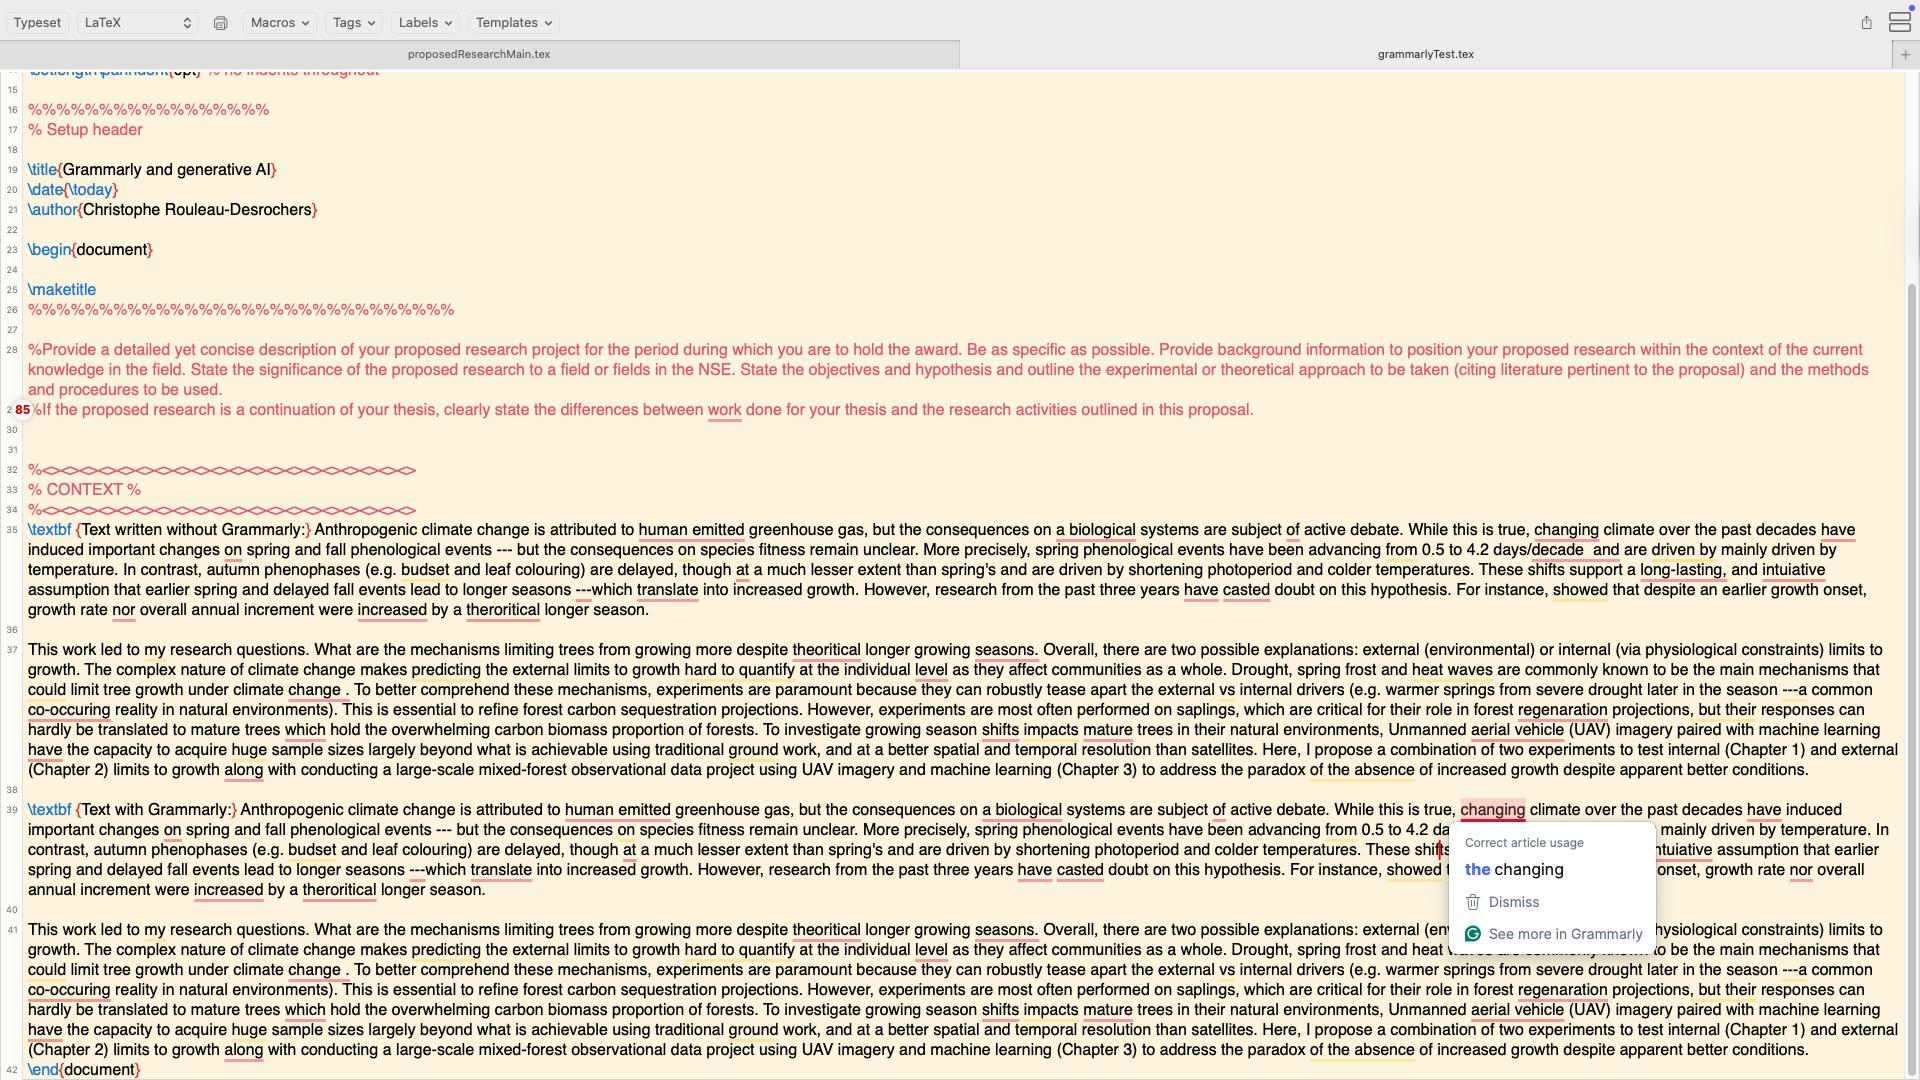
\includegraphics[width=0.8\textwidth]{article.png} 
\end{figure}

\newpage

\subsection{Change spelling aka use the right word}
\begin{figure}[h!] 
    \centering
    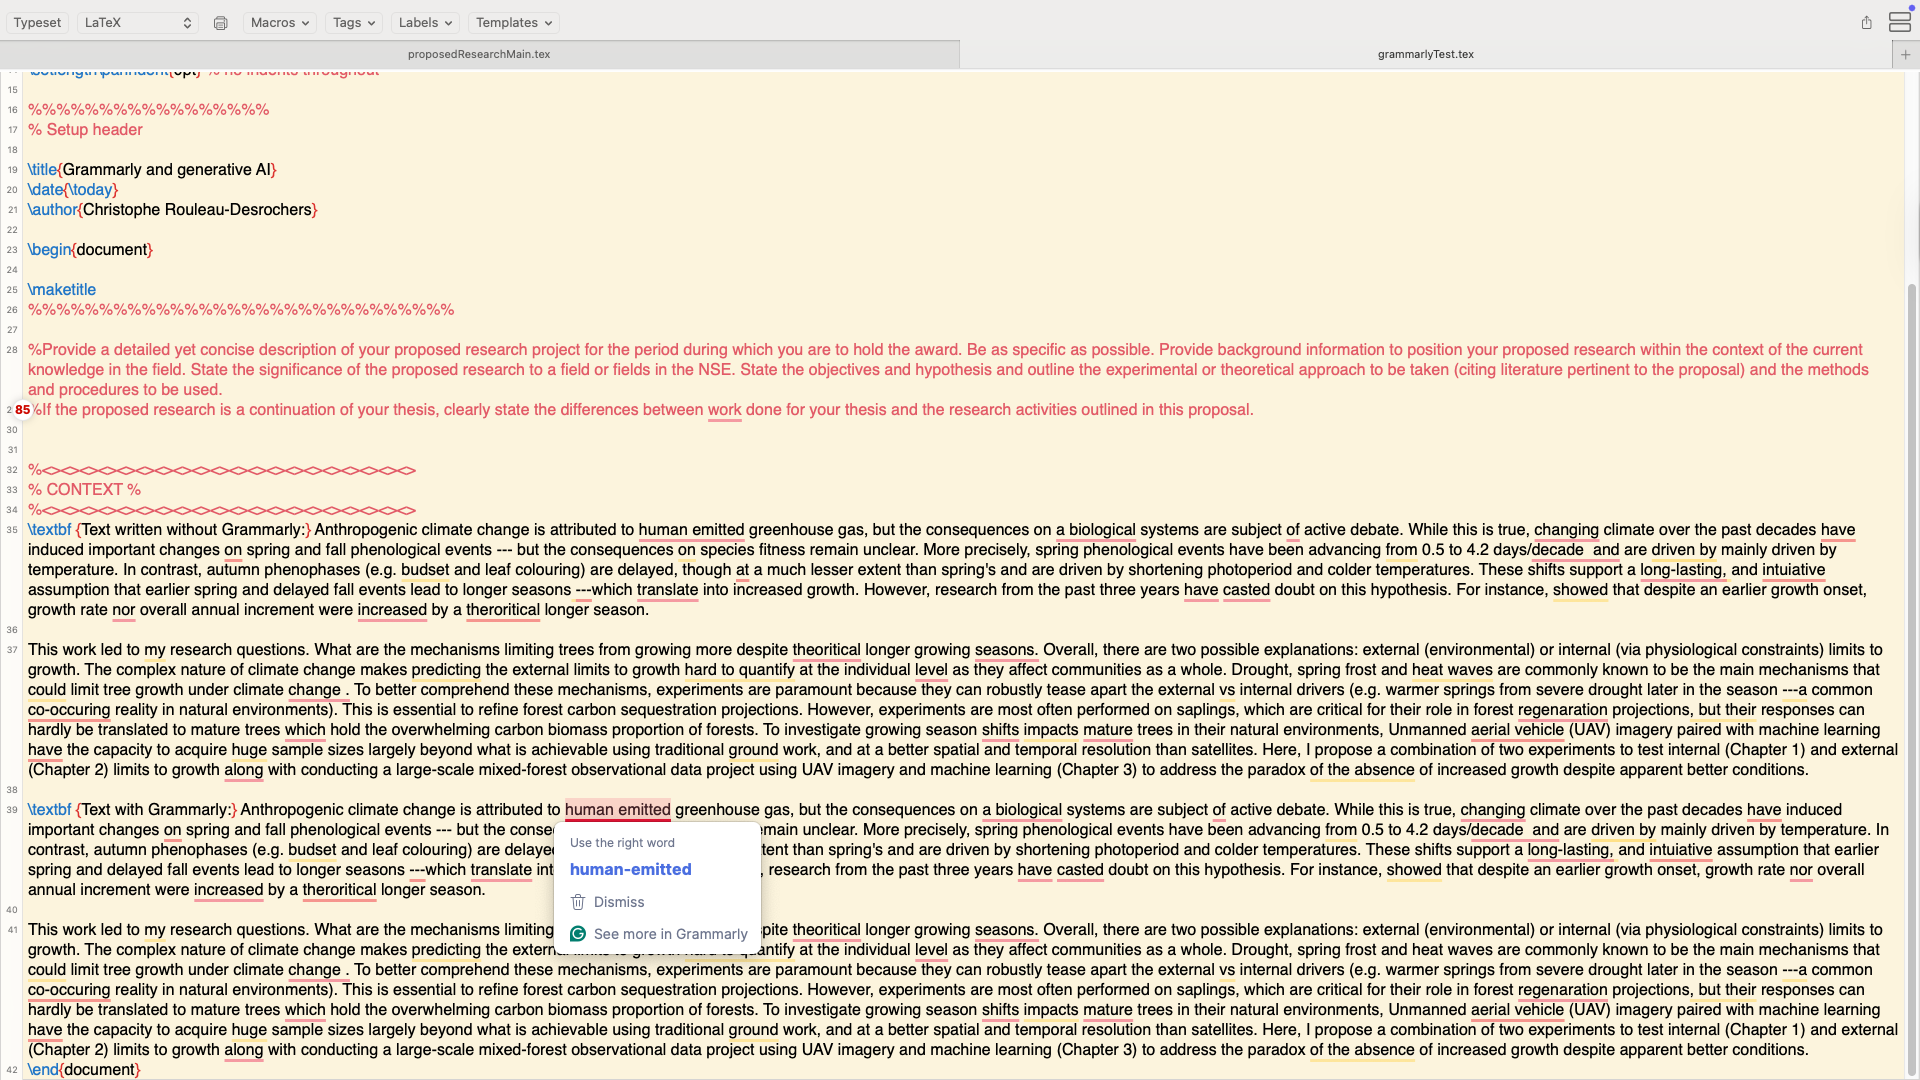
\includegraphics[width=0.8\textwidth]{rightword.png} 
\end{figure}


\subsection{Fix spelling}
\begin{figure}[h!] 
    \centering
    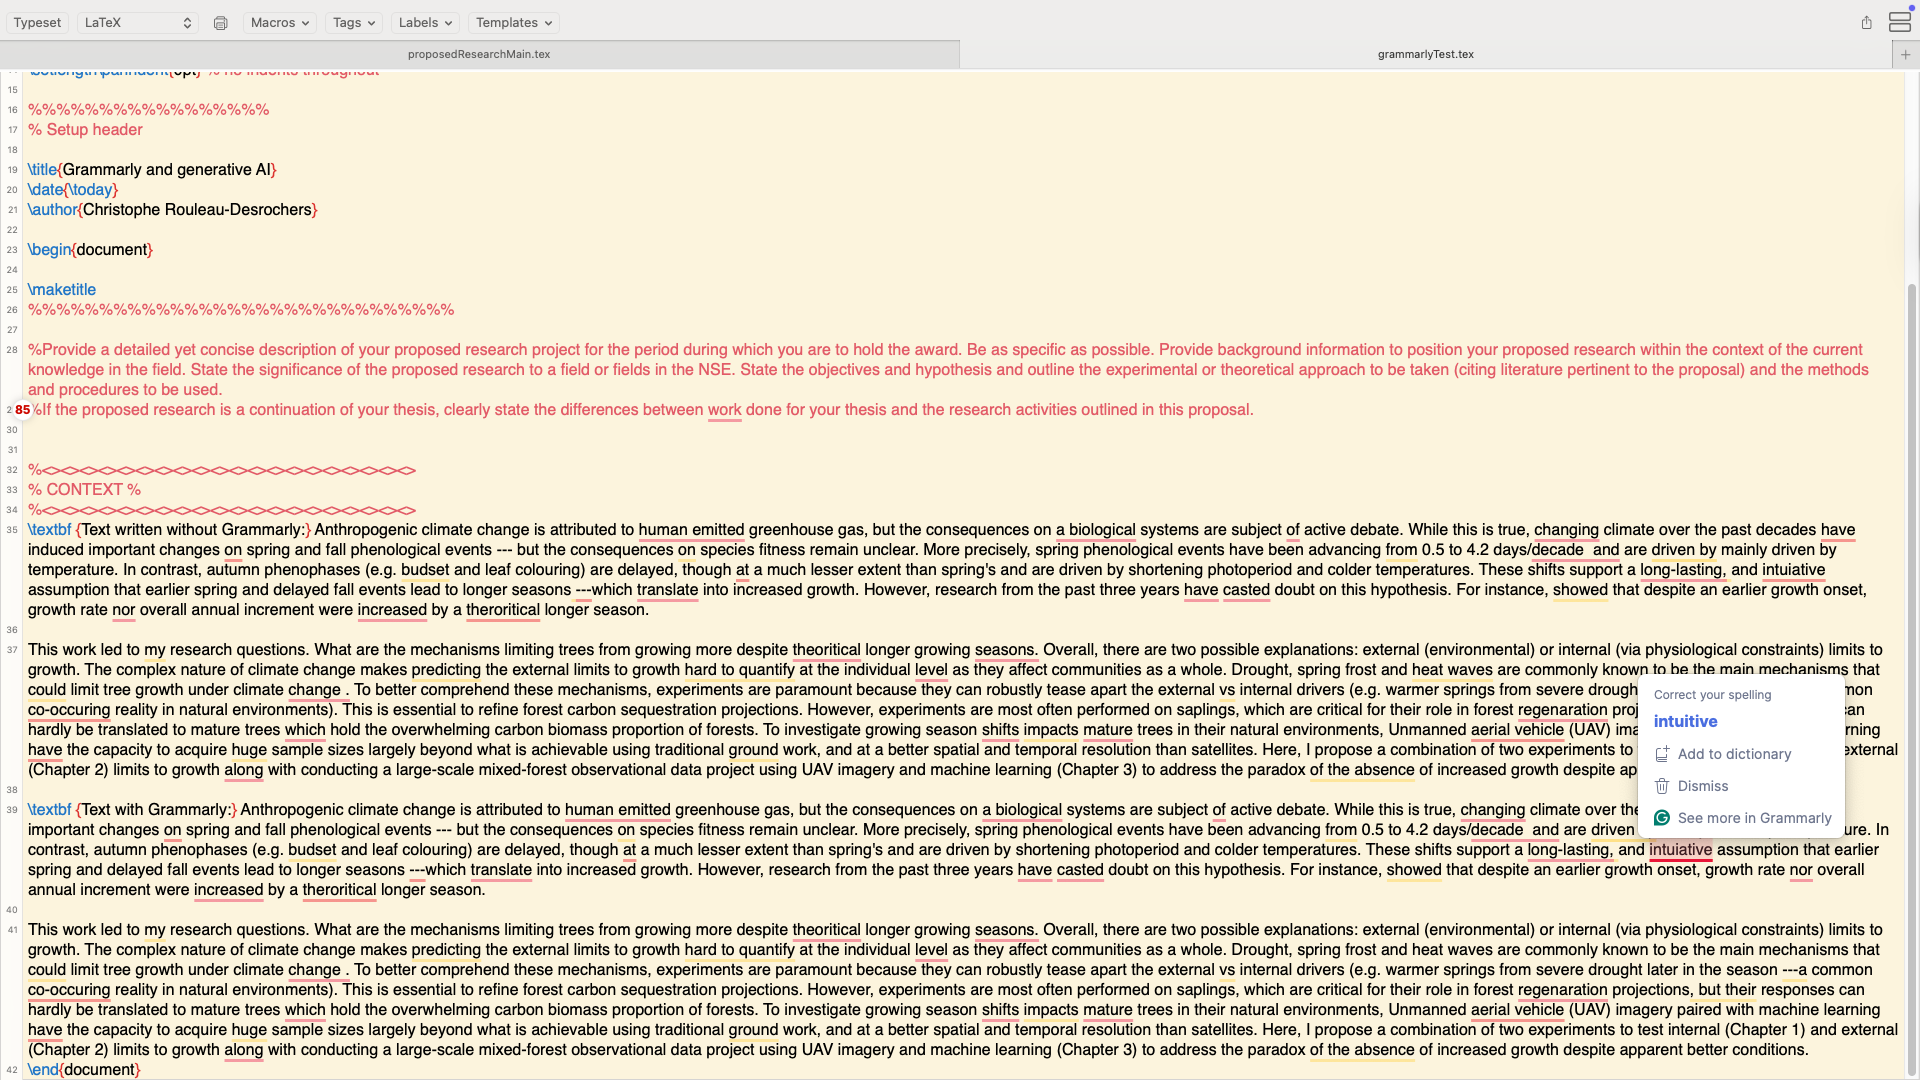
\includegraphics[width=0.8\textwidth]{spelling.png} 
\end{figure}

\newpage

\subsection{Remove extra spaces}
\begin{figure}[h!] 
    \centering
    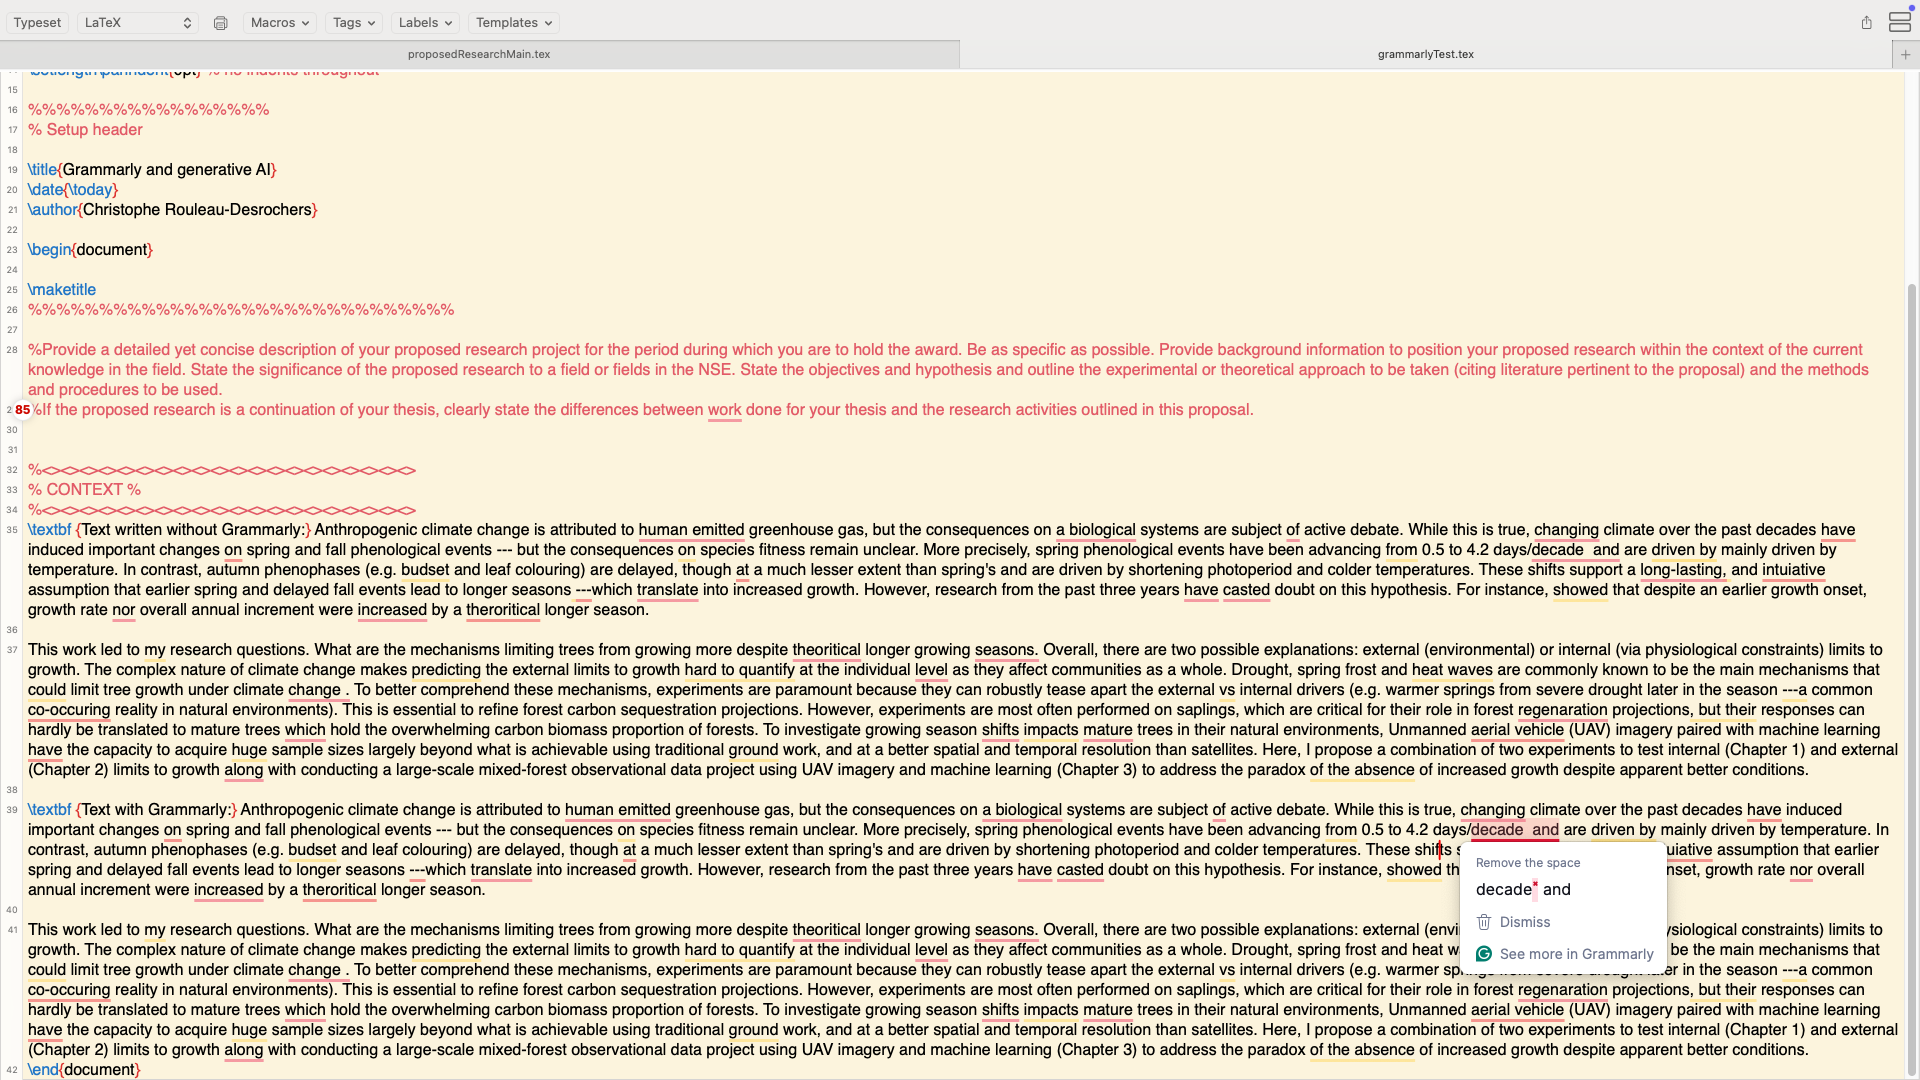
\includegraphics[width=0.8\textwidth]{space.png} 
\end{figure}

\subsection{Subject-verb aggrement}
\begin{figure}[h!] 
    \centering
    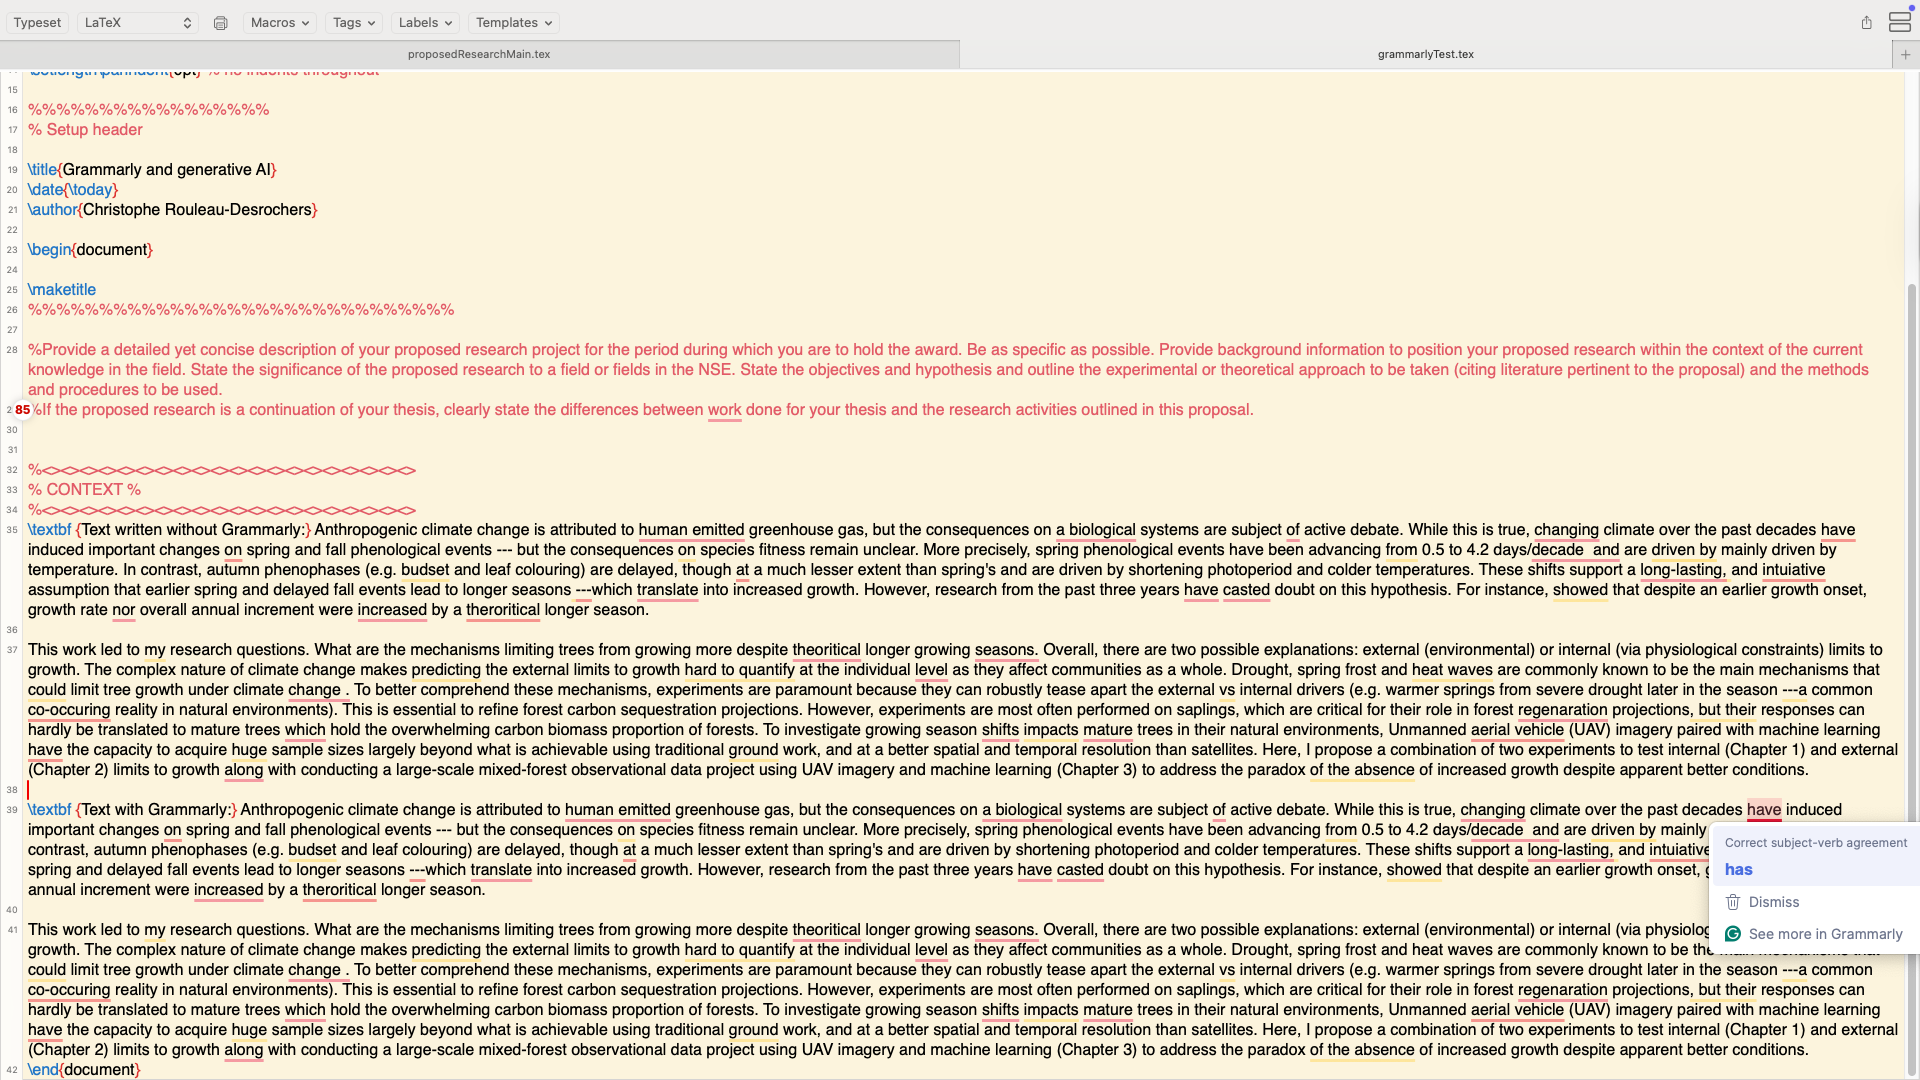
\includegraphics[width=0.8\textwidth]{subjectverbaggrement.png} 
\end{figure}
\newpage
\section{Examples of what I **don't** and won't use Grammarly for}

\subsection{\textit{Smart} suggestions that use generative AI for rewording your sentences}
\begin{figure}[h!] 
    \centering
    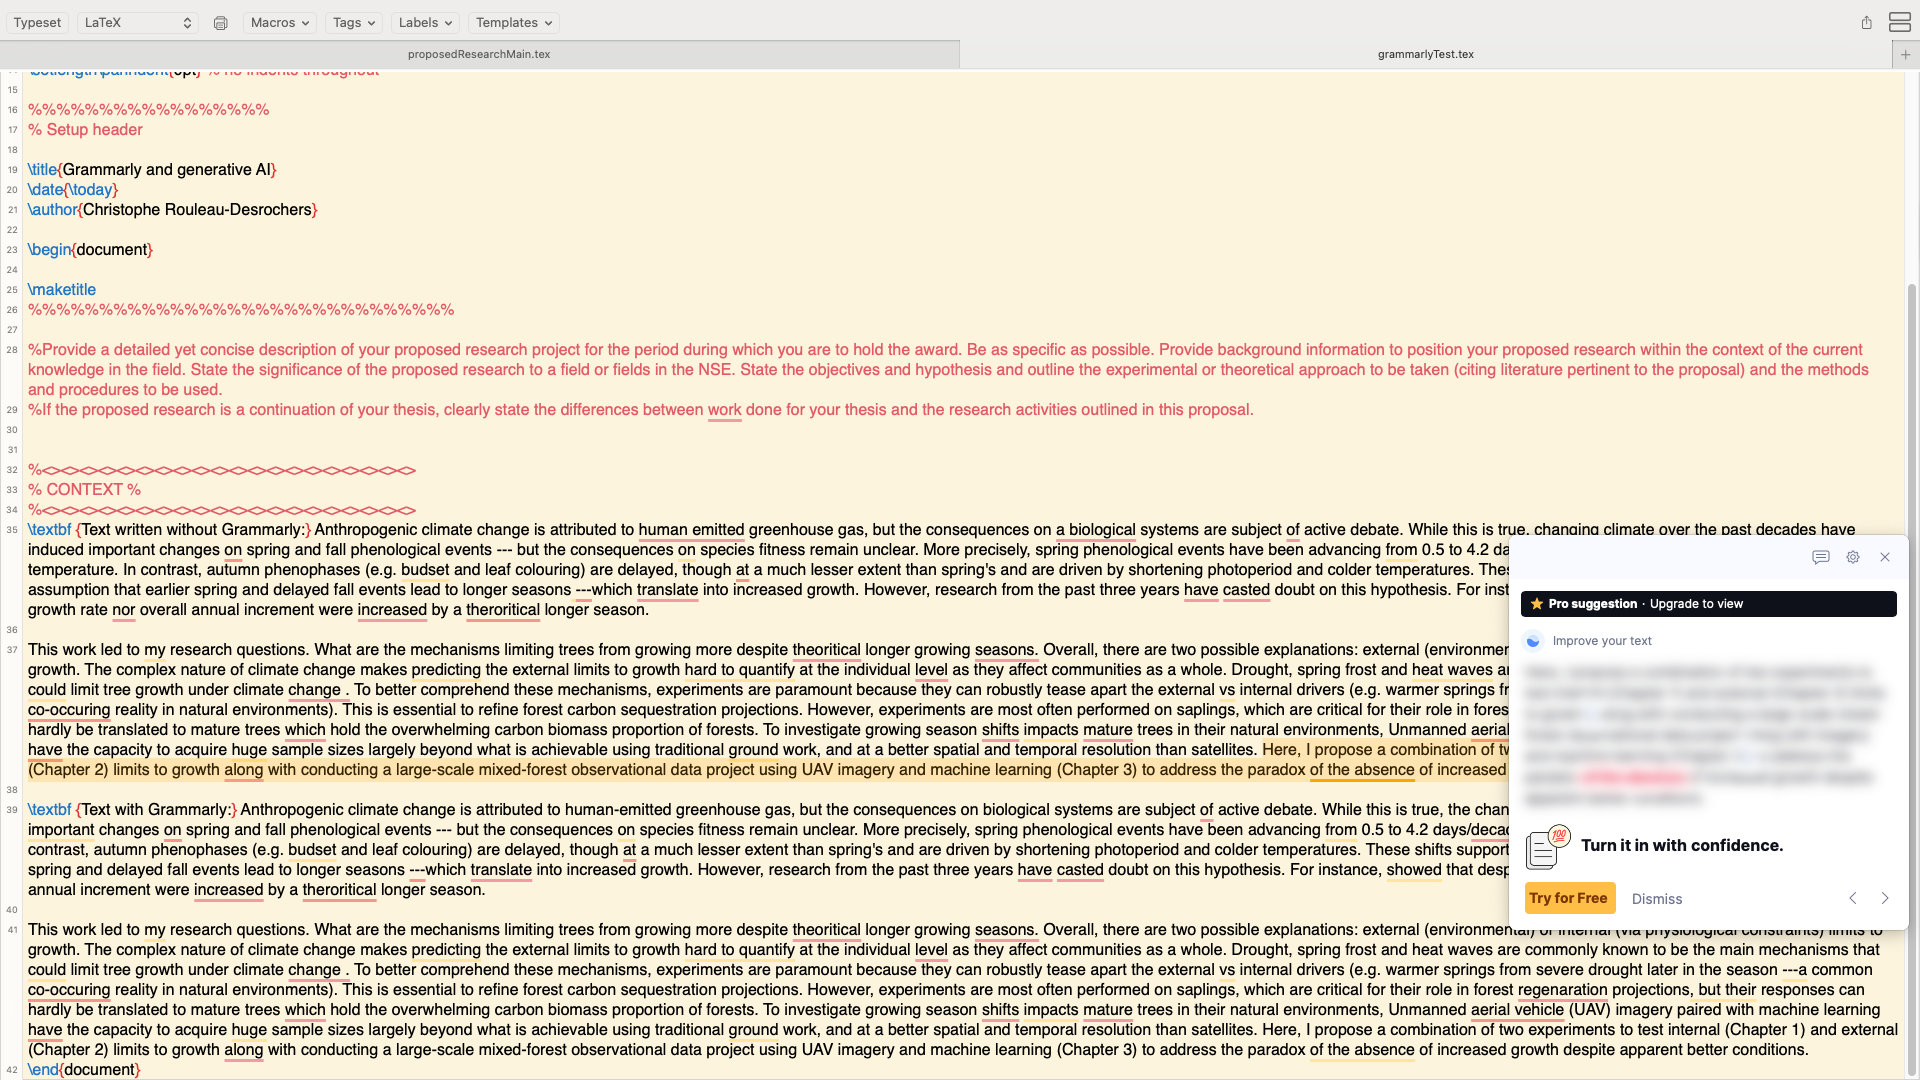
\includegraphics[width=0.8\textwidth]{prosuggestion.png} 
\end{figure}
\newpage
\subsection{\textit{Smart} suggestions that use generative AI for rewording your sentences}
\begin{figure}[h!] 
    \centering
    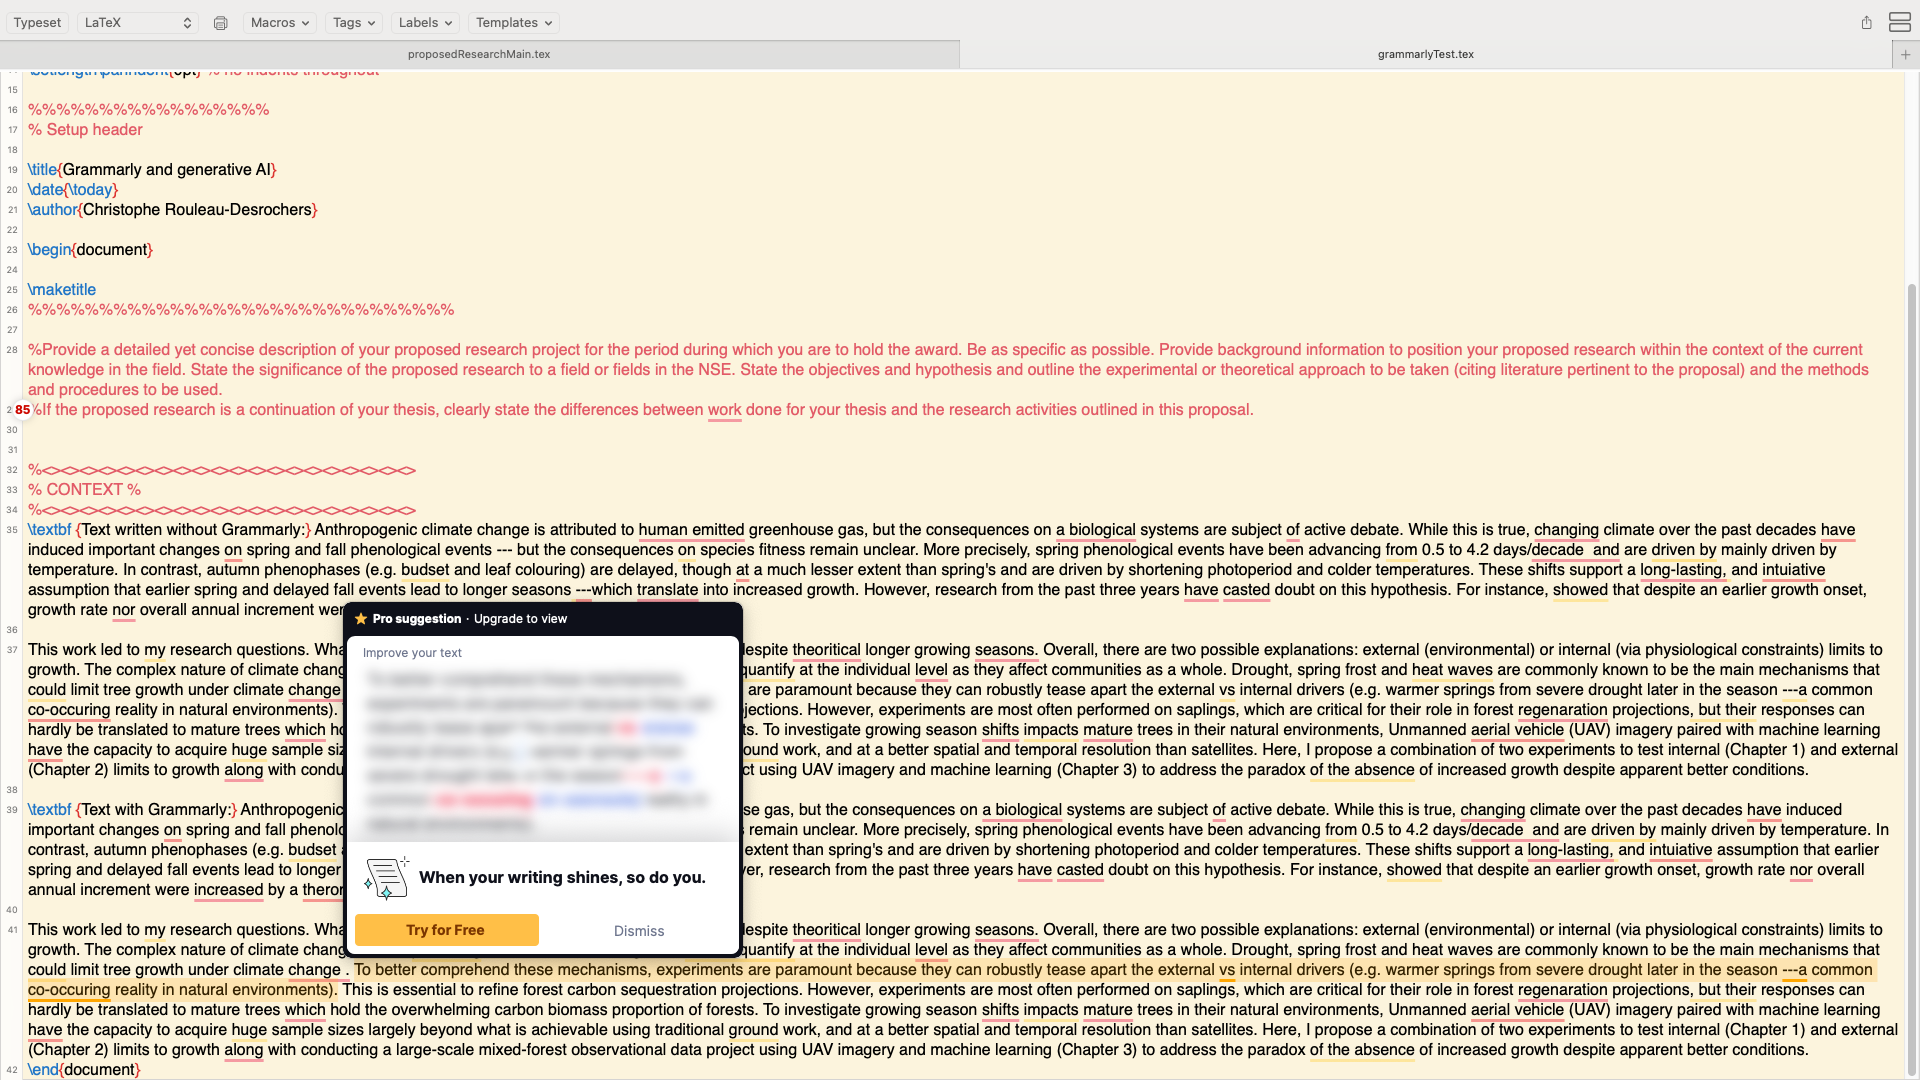
\includegraphics[width=0.8\textwidth]{prosuggestion2.png} 
\end{figure}


\section{Thoughts}
I started going in the rabbit hole of how Grammarly uses AI, and from what I understand, their generative AI model is a paid option that you can get limited access to under the basic version of it (Pro suggestion). The way I've used Grammarly in the past and think it's ok to use it still is to check verb tenses, grammar, punctuation and spelling (basically what is shown in section 1). However, I don't know if these suggestions use generative AI... My suspicion is that it doesn't but I might be wrong. I couldn't find reliable information for this.\\

\section{Before and after spelling and grammar fixes with Grammarly}

\textbf {Text written without Grammarly:} Anthropogenic climate change is attributed to human emitted greenhouse gas, but the consequences on a biological systems are subject of active debate. While this is true, changing climate over the past decades have induced important changes on spring and fall phenological events --- but the consequences on species fitness remain unclear. More precisely, spring phenological events have been advancing from 0.5 to 4.2 days/decade  and are driven by mainly driven by temperature. In contrast, autumn phenophases (e.g. budset and leaf colouring) are delayed, though at a much lesser extent than spring's and are driven by shortening photoperiod and colder temperatures. These shifts support a long-lasting, and intuiative assumption that earlier spring and delayed fall events lead to longer seasons ---which translate into increased growth. However, research from the past three years have casted doubt on this hypothesis. For instance, showed that despite an earlier growth onset, growth rate nor overall annual increment were increased by a theroritical longer season. 

This work led to my research questions. What are the mechanisms limiting trees from growing more despite theoritical longer growing seasons. Overall, there are two possible explanations: external (environmental) or internal (via physiological constraints) limits to growth. The complex nature of climate change makes predicting the external limits to growth hard to quantify at the individual level as they affect communities as a whole. Drought, spring frost and heat waves are commonly known to be the main mechanisms that could limit tree growth under climate change . To better comprehend these mechanisms, experiments are paramount because they can robustly tease apart the external vs internal drivers (e.g. warmer springs from severe drought later in the season ---a common co-occuring reality in natural environments). This is essential to refine forest carbon sequestration projections. However, experiments are most often performed on saplings, which are critical for their role in forest regenaration projections, but their responses can hardly be translated to mature trees which hold the overwhelming carbon biomass proportion of forests. To investigate growing season shifts impacts mature trees in their natural environments, Unmanned aerial vehicle (UAV) imagery paired with machine learning have the capacity to acquire huge sample sizes largely beyond what is achievable using traditional ground work, and at a better spatial and temporal resolution than satellites. Here, I propose a combination of two experiments to test internal (Chapter 1) and external (Chapter 2) limits to growth along with conducting a large-scale mixed-forest observational data project using UAV imagery and machine learning (Chapter 3) to address the paradox of the absence of increased growth despite apparent better conditions. \\
\par
\textbf {Text with Grammarly:} Anthropogenic climate change is attributed to human-emitted greenhouse gas, but the consequences on biological systems are subject to active debate. While this is true, the changing climate over the past decades has induced important changes in spring and fall phenological events --- but the consequences on species fitness remain unclear. More precisely, spring phenological events have been advancing from 0.5 to 4.2 days/decade and are driven by mainly driven by temperature. In contrast, autumn phenophases (e.g. budset and leaf colouring) are delayed, though to a much lesser extent than spring's and are driven by shortening photoperiod and colder temperatures. These shifts support a long-lasting and intuitive assumption that earlier spring and delayed fall events lead to longer seasons-which translate into increased growth. However, research from the past three years has cast doubt on this hypothesis. For instance, Dow 2022 showed that despite an earlier growth onset, growth rate or overall annual increment were increased by a longer theoretical season. 

This work led to my research questions. What are the mechanisms limiting trees from growing more despite theoretically longer growing seasons? Overall, there are two possible explanations: external (environmental) or internal (via physiological constraints) limits to growth. The complex nature of climate change makes predicting the external limits to growth hard to quantify at the individual level, as they affect communities as a whole. Drought, spring frost and heat waves are commonly known to be the main mechanisms that could limit tree growth under climate change. To better comprehend these mechanisms, experiments are paramount because they can robustly tease apart the external vs internal drivers (e.g. warmer springs from severe drought later in the season ---a common co-occurring reality in natural environments). This is essential to refine forest carbon sequestration projections. However, experiments are most often performed on saplings, which are critical for their role in forest regeneration projections, but their responses can hardly be translated to mature trees, which hold the overwhelming carbon biomass proportion of forests. To investigate growing season shifts' impacts on mature trees in their natural environments, Unmanned aerial vehicle (UAV) imagery paired with machine learning has the capacity to acquire huge sample sizes largely beyond what is achievable using traditional ground work, and at a better spatial and temporal resolution than satellites. Here, I propose a combination of two experiments to test internal (Chapter 1) and external (Chapter 2) limits to growth, along with conducting a large-scale mixed-forest observational data project using UAV imagery and machine learning (Chapter 3) to address the paradox of the absence of increased growth despite apparent better conditions.


\end{document}